This section provides a brief introduction to Bitcoin, the
world's first decentralized digital currency. We will begin by exploring
the historical context in which Bitcoin was created, with a particular
focus on the 2008 financial crisis and the erosion of trust in
traditional financial institutions that it engendered. We will then
delve into the fundamental principles that underpin the Bitcoin network,
including its peer-to-peer architecture, the roles of various network
participants, and the structure of transactions and blocks.

A significant portion of this section is dedicated to explaining the key
technological innovations that make Bitcoin possible. We will examine
the Unspent Transaction Output (UTXO) model, which is used to track the
ownership of bitcoins, and the Proof-of-Work (PoW) consensus mechanism,
which secures the network and ensures its integrity. We will also
discuss the challenges that Bitcoin faces, such as its limited
scalability and the privacy concerns associated with its public ledger.
Finally, we will introduce the Lightning Network, a promising Layer 2
solution that aims to address Bitcoin's scalability limitations and
enable fast, low-cost transactions.

\subsection{Learning Objectives}\label{learning-objectives}

\begin{itemize}
	\tightlist
	\item
	Understand the historical context and motivation behind the creation
	of Bitcoin.
	\item
	Grasp the basic concepts of the Bitcoin network, including clients,
	miners, addresses, and transactions.
	\item
	Learn about the structure of the Bitcoin blockchain and the role of
	the Proof-of-Work consensus mechanism.
	\item
	Understand the Unspent Transaction Output (UTXO) model and how it is
	used to track ownership of bitcoins.
	\item
	Gain insight into the challenges facing Bitcoin, such as scalability,
	energy consumption, and privacy.
	\item
	Learn about the Lightning Network as a potential solution to Bitcoin's
	scalability issues.
\end{itemize}

\begin{center}\rule{0.5\linewidth}{0.5pt}\end{center}

\subsection{The History and Genesis of
	Bitcoin}\label{section-1-the-history-and-genesis-of-bitcoin}

\subsubsection{The White Paper and the 2008 Financial
	Crisis}\label{the-white-paper-and-the-2008-financial-crisis}

The genesis of Bitcoin is inextricably linked to the global financial
crisis of 2008. In October of that year, as the crisis was unfolding, a
white paper titled ``Bitcoin: A Peer-to-Peer Electronic Cash System''~\cite{nakamoto2008bitcoin}
was published under the pseudonym Satoshi Nakamoto. The paper proposed a
revolutionary new system for electronic transactions that would operate
without the need for a trusted third party, such as a bank or financial
institution.

The timing of the white paper's release was no coincidence. The 2008
financial crisis, triggered by the collapse of the subprime mortgage
market in the United States, led to a widespread loss of faith in the
traditional financial system. The crisis exposed the systemic risks
inherent in a centralized banking system and the potential for
governments to devalue currencies through inflation. In this climate of
distrust and uncertainty, the idea of a decentralized,
censorship-resistant, and mathematically secured form of money was
particularly appealing.

The Bitcoin white paper laid out the technical foundations for a system
that would allow for direct, peer-to-peer transactions, secured by
cryptographic proof instead of trust. This vision of a new financial
paradigm, free from the control of central authorities, resonated with a
growing community of cryptographers, cypherpunks, and libertarians who
were disillusioned with the existing financial order.

\subsubsection{Satoshi Nakamoto and the Early
	Days}\label{satoshi-nakamoto-and-the-early-days}

The identity of Satoshi Nakamoto remains one of the most enduring
mysteries of the digital age. The name is a pseudonym for the person or
group of people who created Bitcoin. From 2008 to 2011, Nakamoto was an
active participant in the development of Bitcoin, collaborating with
other developers on forums and mailing lists. However, in 2011, Nakamoto
abruptly disappeared, leaving the future of Bitcoin in the hands of the
community.

Despite numerous attempts to uncover the true identity of Satoshi
Nakamoto, it remains unknown. Several individuals have been suggested as
potential candidates, but none have been definitively proven to be the
creator of Bitcoin. The legacy of Satoshi Nakamoto is not just the
Bitcoin protocol and its reference implementation, but also the vision
of a decentralized financial system that has inspired a global movement
and a multi-trillion dollar industry.

\begin{center}\rule{0.5\linewidth}{0.5pt}\end{center}

\subsection{The Basics of Bitcoin}\label{section-2-bitcoin-101-the-basics}

\subsubsection{Key Facts and Figures}\label{key-facts-and-figures}

Bitcoin is defined by a set of core parameters that are hard-coded into
the protocol. These parameters govern the issuance of new bitcoins, the
size of blocks, and the rate at which new blocks are created.

\begin{itemize}
	\tightlist
	\item
	\textbf{Maximum Supply}: The total supply of bitcoin is capped at 21
	million. This fixed supply is a fundamental aspect of Bitcoin's
	monetary policy and is designed to make it a deflationary currency.
	\item
	\textbf{Block Size}: The maximum size of a Bitcoin block is 4
	megabytes (MB). This limit was introduced to prevent spam and
	denial-of-service attacks on the network.
	\item
	\textbf{Consensus Mechanism}: Bitcoin uses the Proof-of-Work (PoW)
	consensus mechanism, which requires miners to expend computational
	energy to create new blocks.
	\item
	\textbf{Block Time}: The Bitcoin protocol is designed to target a
	block time of approximately 10 minutes. This means that a new block is
	added to the blockchain, on average, every 10 minutes.
\end{itemize}

\subsubsection{The Bitcoin Network}\label{the-bitcoin-network}

The Bitcoin network is a global, peer-to-peer (P2P) network of computers
that work together to maintain the integrity of the blockchain. The
network is composed of various types of participants (as we mentioned in \autoref{sec:participants-in-a-blockchain-network}), each with a
specific role:

\begin{itemize}
	\tightlist
	\item
	\textbf{Lightweight Clients, a.k.a., SPV (Simple Payment Verification) Clients}: These are
	lightweight nodes that do not store the entire blockchain. Instead,
	they only download the block headers, which allows them to verify
	transactions with the help of full nodes without having to download
	and process the entire blockchain.
	Note that less secure version of clients are represented by some wallets that rely on a trusted centralized server for providing information about the current state of the blockchain. 
	These are software or hardware
	applications that allow users to store and manage their bitcoins.
	Wallets generate and store the user's private keys, which are required
	to sign transactions and authorize the spending of funds.
	\item
	\textbf{Miners / Consensus Nodes}: These are specialized nodes that are responsible for
	creating new blocks. They do this by collecting pending transactions
	from the network, organizing them into a new block, and then competing
	to solve the Proof-of-Work puzzle. The first miner to solve the puzzle
	is rewarded with newly created bitcoins and the transaction fees from
	the transactions included in the block.
	\item
	\textbf{Full Nodes}: These are nodes that store a complete copy of the
	Bitcoin blockchain. They independently validate all transactions and
	blocks against the protocol's consensus rules, ensuring that all
	participants are adhering to the same set of rules. Full nodes are the
	backbone of the network, providing a high level of security and
	decentralization.


\end{itemize}

\subsubsection{Addresses and
	Transactions}\label{addresses-and-transactions}

\begin{itemize}
	\tightlist
	\item
	\textbf{Addresses}: A Bitcoin address is a unique identifier,
	analogous to an email address, that is used to send and receive
	bitcoins. It is a string of alphanumeric characters that is derived
	from a user's public key using the ECDSA algorithm on the secp256k1
	curve, followed by SHA-256 and RIPEMD-160 hashing.
	\item
	\textbf{Transactions}: A Bitcoin transaction is a digitally signed
	message that authorizes the transfer of value from one address to
	another. A transaction consists of one or more inputs and one or more
	outputs. The inputs are references to unspent outputs from previous
	transactions, and the outputs specify the new owners of the bitcoins
	and the amount they are entitled to spend.
\end{itemize}

\begin{center}\rule{0.5\linewidth}{0.5pt}\end{center}

\subsection{Diving Deeper into the Blockchain and Consensus}\label{section-3-diving-deeper-into-the-blockchain}

\subsubsection{Block Structure and the Merkle
	Tree}\label{block-structure-and-the-merkle-tree}

A Bitcoin block is a data structure that contains a batch of
transactions. It is composed of two main parts: a block header and a
block body (see \autoref{fig:block-structure}). The block body contains the list of transactions that are
included in the block. These transactions are organized into a
\textbf{Merkle tree}, a data structure that allows for efficient
verification of the integrity of the transactions. The root of the
Merkle tree, known as the Merkle root, is included in the block header.

\begin{figure}[t]
	%	\vspace{-0.3cm}
	\begin{center}
		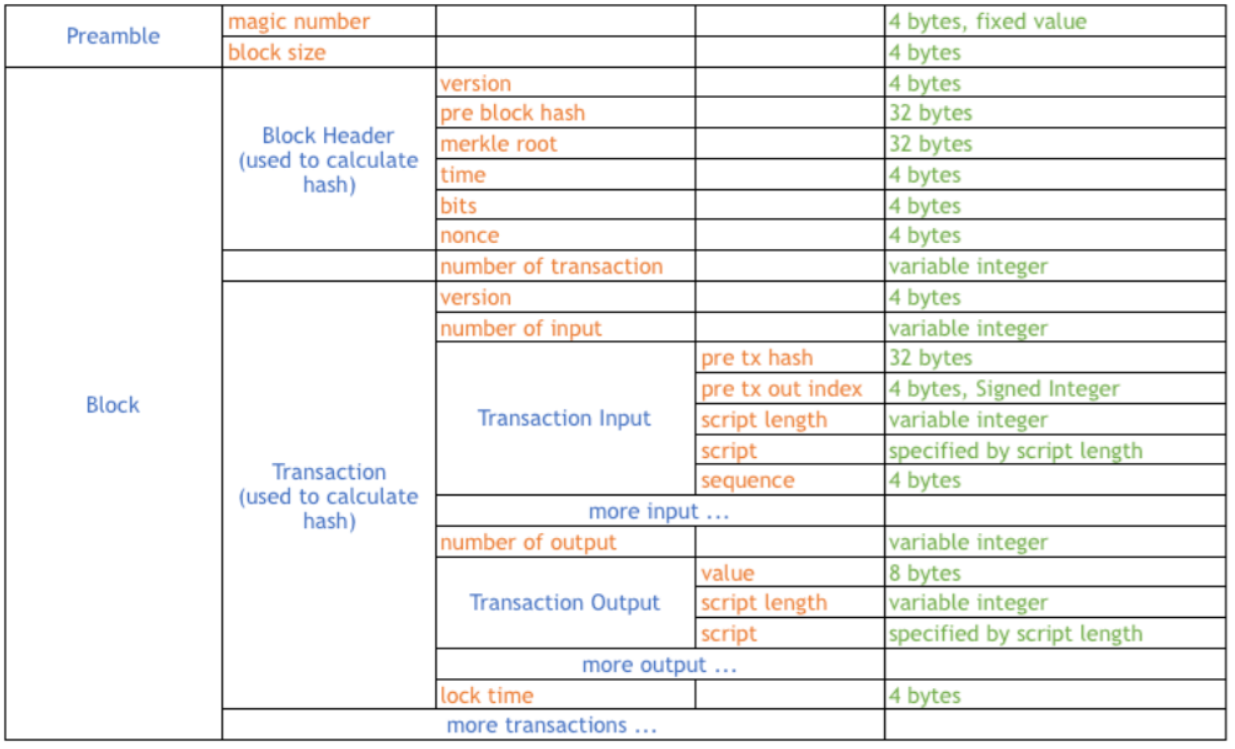
\includegraphics[width=0.9\textwidth]{./figs/block-structructure.png}
		\caption{Bitcoin's block structure~\ih{CITE https://www.blockchain.com/btc/block/100000}.}		
		\label{fig:block-structure}
	\end{center}	
\end{figure}

The block header contains several important pieces of information,
including:

\begin{itemize}
	\tightlist
	\item
	\textbf{Version}: The block version number.
	\item
	\textbf{Previous Block Hash}: The hash of the previous block's header,
	which links the blocks together in a chain.
	\item
	\textbf{Merkle Root}: The root of the Merkle tree of all the
	transactions in the block.
	\item
	\textbf{Timestamp}: The time at which the block was created.
	\item
	\textbf{Difficulty Target}: The target value that the hash of the
	block header must be less than.
	\item
	\textbf{Nonce}: A random value that is incremented by miners in the
	process of finding a valid hash.
\end{itemize}

\subsubsection{Proof-of-Work and Nakamoto's
	Consensus}\label{proof-of-work-and-nakamotos-consensus}

The security of the Bitcoin blockchain is underpinned by the
\textbf{Proof-of-Work (PoW)} consensus mechanism, often referred to as
Nakamoto's consensus. This mechanism ensures that new blocks are added
to the blockchain in a secure and decentralized manner.

In the PoW system, miners compete to solve a computationally intensive
puzzle. This puzzle involves finding a nonce that, when combined with
the other fields in the block header and hashed, produces a hash that is
below a certain target value. The first miner to find a valid hash is
rewarded with newly created bitcoins and the transaction fees from the
transactions included in the block.

The schematic diagram of finding a PoW puzzle of Bitcoin is depicted in \autoref{fig:pow-puzzle-scheme}.
\begin{figure}[t]
	%	\vspace{-0.3cm}
	\begin{center}
		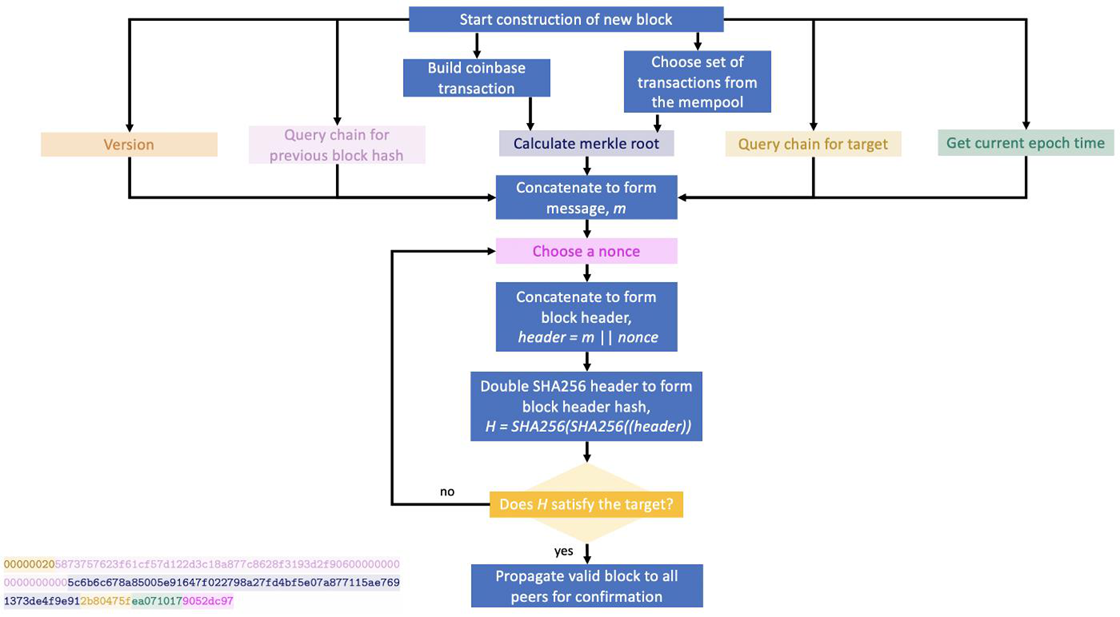
\includegraphics[width=1.1\textwidth]{./figs/pow-scheme.png}
		\caption{Finding a PoW puzzle of Bitcoin~\ih{CITE https://medium.com/fcats-blockchain-incubator/understanding-the-bitcoin-blockchain-header-a2b0db06b515}.}		
		\label{fig:pow-puzzle-scheme}
	\end{center}	
\end{figure}

Also a simplified Python code snippet that demonstrates the
Proof-of-Work algorithm is depicted in \autoref{fig:pow-puzzle-python}.
\begin{figure}[t]
	%	\vspace{-0.3cm}
	\begin{center}
		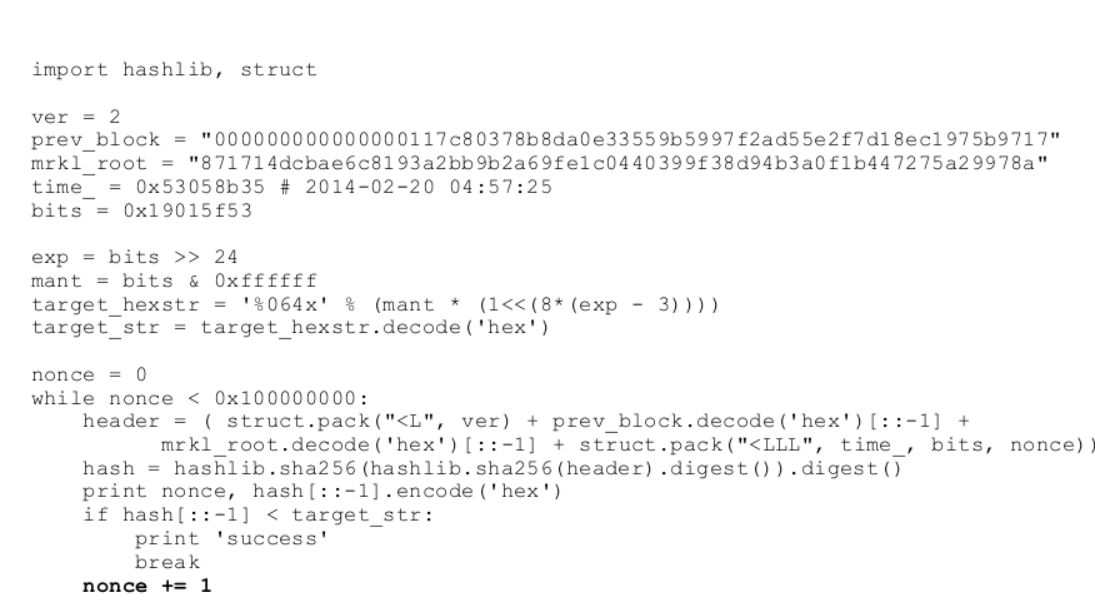
\includegraphics[width=0.9\textwidth]{./figs/pow-python.png}
		\caption{A simplified python code of finding a PoW puzzle in Bitcoin.}		
		\label{fig:pow-puzzle-python}
	\end{center}	
\end{figure}



%\begin{Shaded}
%	\begin{Highlighting}[]
%		\ImportTok{import}\NormalTok{ hashlib, struct}
%		
%		\NormalTok{ver }\OperatorTok{=} \DecValTok{2}
%		\NormalTok{prev\_block }\OperatorTok{=} \StringTok{"000000000000000117c80378b8da0e33559b5997f2ad55e2f7d18ec1975b9717"}
%		\NormalTok{mrkl\_root }\OperatorTok{=} \StringTok{"871714dcbae6c8193a2bb9b2a69fe1c0440399f38d94b3a0f1b447275a29978a"}
%		\NormalTok{time\_ }\OperatorTok{=} \BaseNTok{0x53058b35} \CommentTok{\# 2014{-}02{-}20 04:57:25}
%		\NormalTok{bits }\OperatorTok{=} \BaseNTok{0x19015f53}
%		
%		\NormalTok{exp }\OperatorTok{=}\NormalTok{ bits }\OperatorTok{\textgreater{}\textgreater{}} \DecValTok{24}
%		\NormalTok{mant }\OperatorTok{=}\NormalTok{ bits }\OperatorTok{\&} \BaseNTok{0xffffff}
%		\NormalTok{target\_hexstr }\OperatorTok{=} \StringTok{\textquotesingle{}}\SpecialCharTok{\%064x}\StringTok{\textquotesingle{}} \OperatorTok{\%}\NormalTok{ (mant }\OperatorTok{*}\NormalTok{ (}\DecValTok{1}\OperatorTok{\textless{}\textless{}}\NormalTok{(}\DecValTok{8}\OperatorTok{*}\NormalTok{(exp }\OperatorTok{{-}} \DecValTok{3}\NormalTok{))))}
%		\NormalTok{target\_str }\OperatorTok{=}\NormalTok{ target\_hexstr.decode(}\StringTok{\textquotesingle{}hex\textquotesingle{}}\NormalTok{)}
%		
%		\NormalTok{nonce }\OperatorTok{=} \DecValTok{0}
%		\ControlFlowTok{while}\NormalTok{ nonce }\OperatorTok{\textless{}} \BaseNTok{0x100000000}\NormalTok{:}
%		\NormalTok{    header }\OperatorTok{=}\NormalTok{ ( struct.pack(}\StringTok{"\textless{}L"}\NormalTok{, ver) }\OperatorTok{+}\NormalTok{ prev\_block.decode(}\StringTok{\textquotesingle{}hex\textquotesingle{}}\NormalTok{)[::}\OperatorTok{{-}}\DecValTok{1}\NormalTok{] }\OperatorTok{+}
%		\NormalTok{    mrkl\_root.decode(}\StringTok{\textquotesingle{}hex\textquotesingle{}}\NormalTok{)[::}\OperatorTok{{-}}\DecValTok{1}\NormalTok{] }\OperatorTok{+}\NormalTok{ struct.pack(}\StringTok{"\textless{}LLL"}\NormalTok{, time\_, bits, nonce))}
%		\BuiltInTok{hash} \OperatorTok{=}\NormalTok{ hashlib.sha256(hashlib.sha256(header).digest()).digest()}
%		\BuiltInTok{print}\NormalTok{ nonce, }\BuiltInTok{hash}\NormalTok{[::}\OperatorTok{{-}}\DecValTok{1}\NormalTok{].encode(}\StringTok{\textquotesingle{}hex\textquotesingle{}}\NormalTok{)}
%		\ControlFlowTok{if} \BuiltInTok{hash}\NormalTok{[::}\OperatorTok{{-}}\DecValTok{1}\NormalTok{] }\OperatorTok{\textless{}}\NormalTok{ target\_str:}
%		\BuiltInTok{print} \StringTok{\textquotesingle{}success\textquotesingle{}}
%		\ControlFlowTok{break}
%		\NormalTok{    nonce }\OperatorTok{+=} \DecValTok{1}
%	\end{Highlighting}
%\end{Shaded}

The \textbf{difficulty} of the mining puzzle is a critical parameter
that is adjusted every 2016 blocks (approximately every two weeks) to
maintain a consistent block time of around 10 minutes. If blocks are
being created too quickly, the difficulty is increased. If they are
being created too slowly, the difficulty is decreased. This ensures that
the rate of new bitcoin issuance remains predictable and that the
network remains secure.

\subsubsection{The Coinbase Transaction and the Genesis
	Block}\label{the-coinbase-transaction-and-the-genesis-block}

The first transaction in every block is a special transaction known as
the \textbf{coinbase transaction}. This transaction is created by the
miner who successfully mined the block and has two main purposes:

\begin{enumerate}
	\def\labelenumi{\arabic{enumi}.}
	\tightlist
	\item
	\textbf{Block Reward}: It allows the miner to claim the block reward,
	which is a certain number of newly created bitcoins. The block reward
	is halved approximately every four years in an event known as the
	``halving.''
	\item
	\textbf{Transaction Fees}: It allows the miner to collect the
	transaction fees from all the other transactions included in the
	block.
\end{enumerate}

The very first block in the Bitcoin blockchain, block 0, is known as the
\textbf{Genesis Block}. It was created by Satoshi Nakamoto on January 3,
2009. The coinbase transaction of the Genesis Block contains a
now-famous message: ``\textit{The Times 03/Jan/2009 Chancellor on brink of
second bailout for banks}.'' This message is widely interpreted as a
commentary on the instability of the traditional financial system and a
statement of intent for Bitcoin as a decentralized alternative.

\begin{center}\rule{0.5\linewidth}{0.5pt}\end{center}

\subsection{The UTXO Model}\label{section-4-the-utxo-model}

\subsubsection{Unspent Transaction Outputs
	(UTXOs)}\label{unspent-transaction-outputs-utxos}

Unlike traditional banking systems that use an account-based model,
Bitcoin uses the \textbf{Unspent Transaction Output (UTXO)} model to
track the ownership of funds. In the UTXO model, a user's balance is not
stored as a single value in an account. Instead, it is the sum of all
the individual, unspent transaction outputs that are locked to the
user's address.

\begin{figure}[t]
	%	\vspace{-0.3cm}
	\begin{center}
		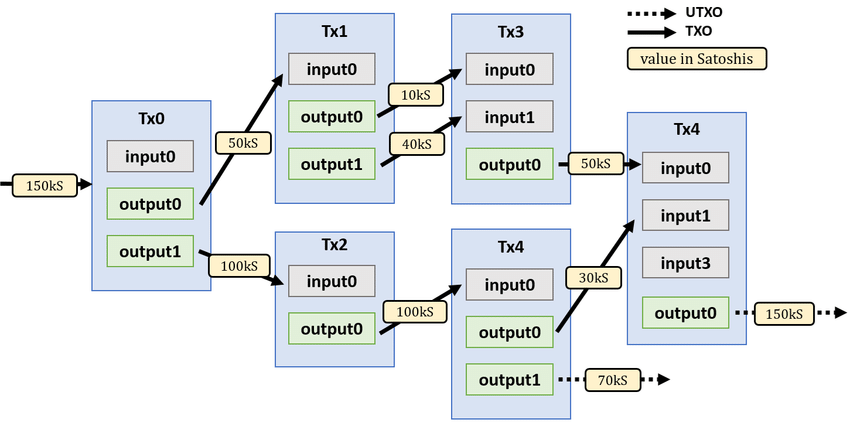
\includegraphics[width=0.9\textwidth]{./figs/utxo.png}
		\caption{Example of UTXO spending.}		
		\label{fig:utxo}
	\end{center}	
\end{figure}

A UTXO is an output of a transaction that has not yet been spent and can
be used as an input in a future transaction. Each UTXO is a discrete
amount of bitcoin that is associated with a specific address. When a
user wants to send bitcoins, their wallet selects a set of UTXOs that
are sufficient to cover the amount of the transaction. These UTXOs are
then used as inputs in the new transaction (see \autoref{fig:utxo}), and new UTXOs are created as
outputs, which are locked to the recipient's address.

Every full node in the Bitcoin network maintains a database of all the
currently unspent transaction outputs, known as the \textbf{UTXO set}. This
database is used to validate new transactions and to ensure that users
can only spend bitcoins that they actually own.

\subsubsection{Transaction Fees and Change
	Outputs}\label{transaction-fees-and-change-outputs}

\begin{itemize}
	\tightlist
	\item
	\textbf{Transaction Fees}: To incentivize miners to include their
	transactions in a block, users can include a transaction fee. The fee
	is the difference between the total value of the inputs and the total
	value of the outputs of a transaction. Miners will typically
	prioritize transactions with higher fees, as this increases their
	profitability.
	\item
	\textbf{Change Outputs}: If the total value of the UTXOs used as
	inputs in a transaction is greater than the amount the user wants to
	send, the excess amount is sent back to the user in a new UTXO, known
	as a \textbf{change output}. This is analogous to receiving change
	when paying for something with cash.
\end{itemize}

\subsubsection{Double-Spending}\label{double-spending}
Double-spending is the act of attempting to spend the same UTXO in more
than one transaction of two or more different temporary or malicious forks. The Bitcoin protocol is designed to prevent
double-spending by ensuring that only one of the conflicting
transactions can be included in the blockchain. Once a transaction is
included in a block and confirmed by the network, the UTXOs it uses as
inputs are considered spent and cannot be used again. Any subsequent
transaction that attempts to spend the same UTXOs will be rejected by
the network as invalid.

\begin{center}\rule{0.5\linewidth}{0.5pt}\end{center}

\subsection{The Lightning Network: A Scalability
	Solution}\label{section-5-the-lightning-network-a-scalability-solution}

One of the most significant challenges facing Bitcoin is its limited
scalability. The combination of a 4 MB block size limit and a 10-minute block time restricts the network's
transaction throughput to approximately 7 transactions per second. This
is a major bottleneck that prevents Bitcoin from being used as a global
payment system for everyday transactions, which would require a much
higher throughput.

\subsubsection{The Lightning Network}\label{the-lightning-network}

The Lightning Network is a Layer 2 scaling solution that is designed to
address Bitcoin's scalability limitations. It is a decentralized network
of off-chain payment channels that allows for instant, low-cost
transactions.

The core idea behind the Lightning Network is to move the majority of
transactions off the main Bitcoin blockchain. Users can open payment
channels with each other by committing a certain amount of bitcoin to a
multi-signature address. Once a channel is open, the two parties can
transact with each other an unlimited number of times without having to
broadcast each transaction to the main blockchain. In this way pairwise network is formed and LN transactions can be route through intermediaries that have sufficient channel capacity (see \autoref{fig:ln}) -- in turn these intermediaries earn routing fees. This allows for instant and virtually free transactions.

\begin{figure}[t]
	%	\vspace{-0.3cm}
	\begin{center}
		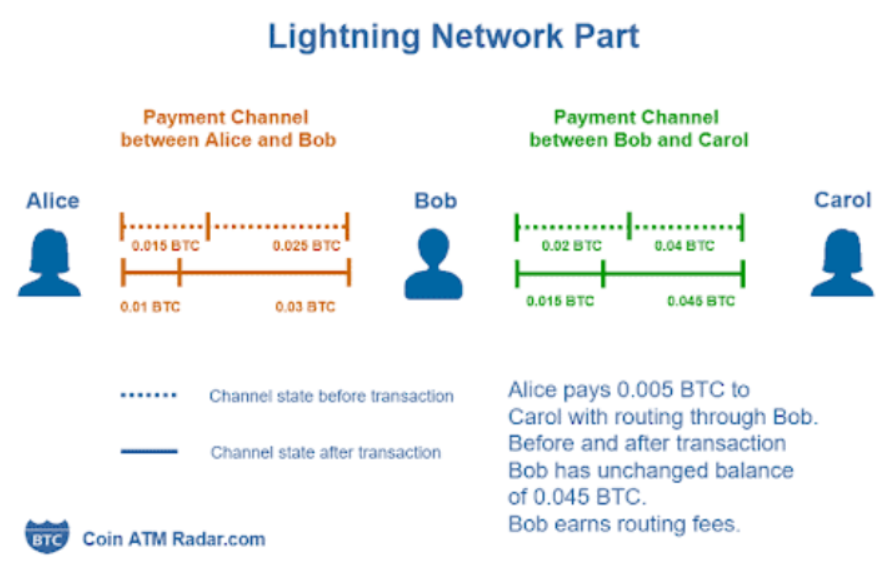
\includegraphics[width=0.9\textwidth]{./figs/ln.png}
		\caption{Lightning network routing and channel update (i.e., balance change).}		
		\label{fig:ln}
	\end{center}	
\end{figure}

The main blockchain is only used to open and close the payment channels.
When the two parties decide to close the channel, the final balance is
settled on the Bitcoin blockchain.

The Lightning Network uses a clever mechanism called \textbf{Hashed
	Time-Locked Contracts (HTLCs)} to enable trustless, multi-hop payments
across the network. This means that two users can transact with each
other even if they do not have a direct payment channel, as long as
there is a path of connected channels between them. In particular, hash time locks enable to conditionally redeem funds by recipient from the sender's output if the pre-image of a hash is revealed in specified time windows. If it is not revealed the funds can be redeemed back by the sender.

\begin{center}\rule{0.5\linewidth}{0.5pt}\end{center}

\subsection{Summary / Key Takeaways}\label{summary-key-takeaways}

This section has provided a detailed introduction to the world of
Bitcoin, the first and most prominent cryptocurrency. We have explored
its origins in the context of the 2008 financial crisis, its core
principles of decentralization and censorship resistance, and the key
technological components that make it function.

We have delved into the peer-to-peer architecture of the Bitcoin
network, identifying the various roles of its participants, from clients
and full nodes to miners. We have also examined the structure of Bitcoin
transactions and blocks, and the crucial role of the Merkle tree in
ensuring data integrity.

A key focus of this section has been the UTXO model, which is Bitcoin's
unique approach to tracking the ownership of funds. We have also
explored the Proof-of-Work consensus mechanism, which is the engine that
secures the Bitcoin blockchain and ensures its immutability.

Finally, we have acknowledged the challenges that Bitcoin faces,
particularly in the areas of scalability and privacy, and we have
introduced the Lightning Network as a promising Layer 2 solution that
aims to address these challenges. This section has laid the groundwork
for a deeper understanding of more advanced topics in blockchain
technology and decentralized applications.

\begin{center}\rule{0.5\linewidth}{0.5pt}\end{center}

\subsection{Keywords}\label{keywords}

\begin{itemize}
	\tightlist
	\item
	\textbf{Bitcoin}: A decentralized digital currency that enables
	peer-to-peer transactions without the need for a central authority.
	\item
	\textbf{Proof-of-Work (PoW)}: A consensus mechanism that secures a
	blockchain by requiring participants to solve a computationally
	intensive puzzle.
	\item
	\textbf{UTXO (Unspent Transaction Output)}: The fundamental building
	block of a Bitcoin transaction, representing a discrete amount of
	bitcoin that can be spent.
	\item
	\textbf{Mining}: The process of creating new blocks in a Proof-of-Work
	blockchain by solving the computational puzzle.
	\item
	\textbf{Lightning Network}: A Layer 2 payment protocol that operates
	on top of the Bitcoin blockchain, enabling fast and low-cost
	transactions.
	\item
	\textbf{Satoshi Nakamoto}: The pseudonymous creator of Bitcoin.
	\item
	\textbf{Genesis Block}: The first block in the Bitcoin blockchain.
	\item
	\textbf{Coinbase Transaction}: A special transaction in each block
	that rewards the miner with newly created bitcoins and transaction
	fees.
	\item
	\textbf{Double-Spending}: The act of spending the same UTXO in
	multiple transactions.
	\item
	\textbf{Hashed Time-Locked Contract (HTLC)}: A type of smart contract
	used in the Lightning Network to enable trustless, multi-hop payments.
\end{itemize}

\begin{center}\rule{0.5\linewidth}{0.5pt}\end{center}

\subsection{Further Reading}\label{further-reading}

\begin{itemize}
	\tightlist
	\item
	\textbf{Bitcoin: A Peer-to-Peer Electronic Cash System}:\\
	\url{https://bitcoin.org/bitcoin.pdf}
	\item
	\textbf{Bitcoin Developer Guide}:\\
	\url{https://bitcoin.org/en/developer-guide}
	\item
	\textbf{Mastering Bitcoin by Andreas M. Antonopoulos}:\\
	\url{https://github.com/bitcoinbook/bitcoinbook}
\end{itemize}
